\subsection{3-1 Differentiate}

\subsubsection{3-1-1 TestDifferentiate}

\subsubsection*{Code}

\inputgroovy[label=Differentiate.groovy,firstline=7]{../ChapterExercises/src/c3/Differentiate.groovy}
\inputgroovy[label=Minus.groovy,firstline=6]{../ChapterExercises/src/c3/Minus.groovy}
\inputgroovy[label=TestDifferentiate.groovy,firstline=6]{../ChapterExercises/src/c3/TestDifferentiate.groovy}

\subsubsection*{Results}

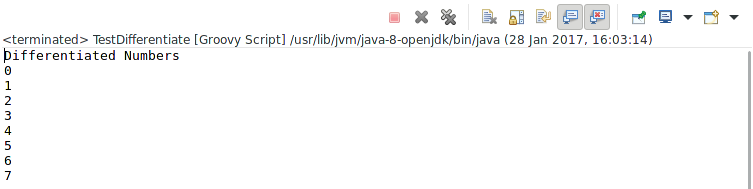
\includegraphics[width=\textwidth]{img/screenshots/3-1-1.png}

\subsubsection{3-1-2 TestDifferentiateNeg}

\subsubsection*{Code}

\inputgroovy[label=DifferentiateNeg.groovy,firstline=6]{../ChapterExercises/src/c3/DifferentiateNeg.groovy}
\inputgroovy[label=Negator.groovy,firstline=4]{../ChapterExercises/src/c3/Negator.groovy}
\inputgroovy[label=TestDifferentiateNeg.groovy,firstline=6]{../ChapterExercises/src/c3/TestDifferentiateNeg.groovy}

\subsubsection*{Results}

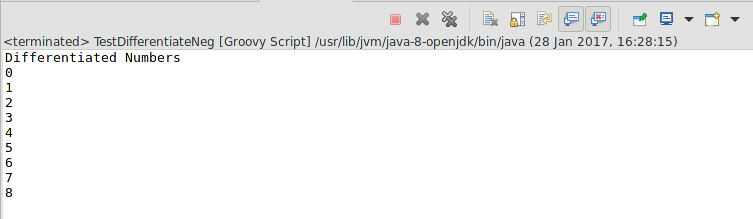
\includegraphics[width=\textwidth]{img/screenshots/3-1-2.png}

\subsubsection*{Questions}

\paragraph{Which is the more pleasing solution? Why?}

Personally I found the first solution, swapping Plus for Minus, the more pleasing solution.  This solution swaps out one of the processes whereas the second solution introduces another process to the mix.  While the overhead of a process is small, it is still there, and unnecessary overhead should be avoided if possible.
